\documentclass[thesis.tex]{subfiles}
\newcommand\TPR{\mathit{TPR}}
\newcommand\FPR{\mathit{FPR}}
\newcommand\OMP{\mathit{1-P}}
\newcommand\TP{\mathit{TP}}
\newcommand\FP{\mathit{FP}}
\newcommand\TN{\mathit{TN}}
\newcommand\FN{\mathit{FN}}
\newcommand\ROC{ROC}
\newcommand\PR{PR}
\begin{document}

\chapter{Methods}

\section{Gaussian scale-space}
\label{sec:GaussianScaleSpace}
%
When taking pictures of the real world, the resulting images are of various sizes and resolutions, and include objects at different distances. This causes details to be present in the images at various scales. Using the Gaussian scale-space representation \cite{griffin1997scale,ginneken2000applications} described in this section, we are able to create a multi-scale representation of the details in an image. The representation consists of a set of smoothed versions of the original image, obtained by applying Gaussian filters $G$ of various sizes $\sigma$ corresponding to the image scales. For a point $(x,y)$, the filter at scale $\sigma$ is defined as
%
\begin{align}
	G(x,y;\sigma) &= \frac{1}{2\pi \sigma^2} \exp \left(\frac{-(x^2+y^2)}{2\sigma^2} \right)
\end{align}
%
and the corresponding scale-space image $L(x,y;\sigma)$ is defined as
%
\begin{align}
	L(x,y;\sigma) &= G(x,y;\sigma) \ast I(x,y),\hspace{1cm}\sigma > 0
\end{align}
%
where $I(x,y)$ is the intensity of the original image $I$ in $(x,y)$ and $\ast$ denotes the convolution operator defined as
\begin{align*}
	f(x,y) \ast g(x,y) &= \int\limits_{\tau_1 = -\infty}^\infty \int\limits_{\tau_2 = -\infty}^\infty f(\tau_1,\tau_2) \cdot g(x-\tau_1,y-\tau_2)\,\text{d}\tau_1\,\text{d}\tau_2
\end{align*}
for the two functions $f$ and $g$ \cite[p.~345]{gonzalez:2008:digital}.

Note that while these scale-space functions are defined on an infinite continuum, in practice we select a finite set of scales for which we wish to retrieve structural information in an image.

\Cref{fig:scaleSpaceExample} shows an example of a finite scale-space representation of an image using the five scales $\sigma = 1,2,4,8,16$. At smaller scales ($\sigma = 1,2$) we are still able to see detailed structure in the gates, pavement, car, hedge, etc. When increasing the scale to $\sigma = 4$, the small details are smoothed out and only the larger details of the mentioned objects are noticeable. At $\sigma = 8, 16$ the details are completely smoothed out and only the larger overall structures are visible. This example clearly shows the power of the scale-space representation being able to model both small details as well as larger structures.
%
\begin{figure}[p]
	\centering
	\begin{subfigure}[t]{0.3\textwidth}
		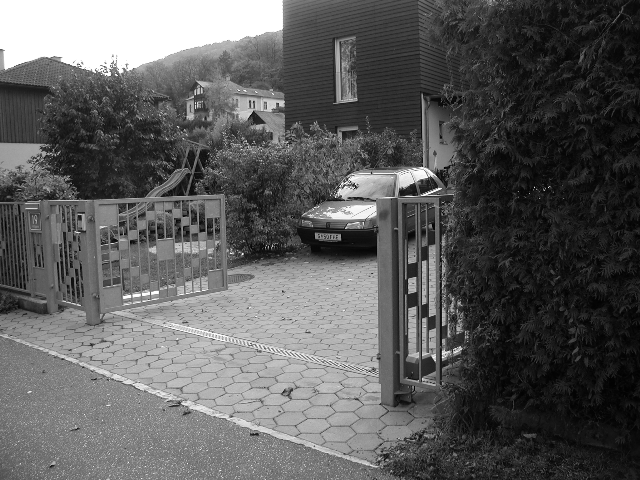
\includegraphics[width=\textwidth]{img/scaleSpaceTheory_0.png}
		\caption{Original}
		\label{fig:scaleSpaceExample0}
	\end{subfigure}
	\begin{subfigure}[t]{0.3\textwidth}
		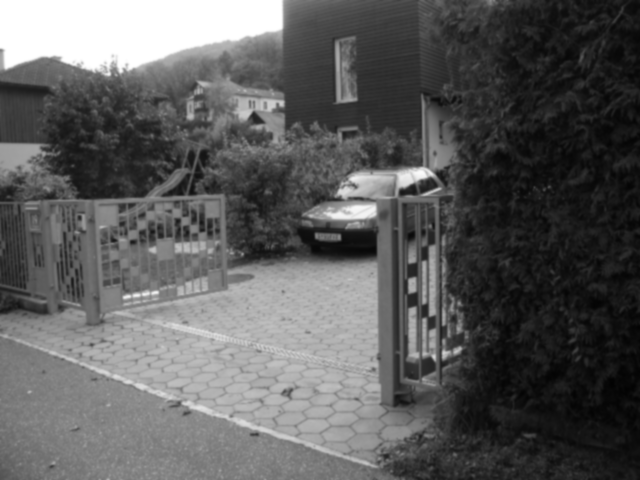
\includegraphics[width=\textwidth]{img/scaleSpaceTheory_1.png}
		\caption{$\sigma = 1$}
		\label{fig:scaleSpaceExample1}
	\end{subfigure}
	\begin{subfigure}[t]{0.3\textwidth}
		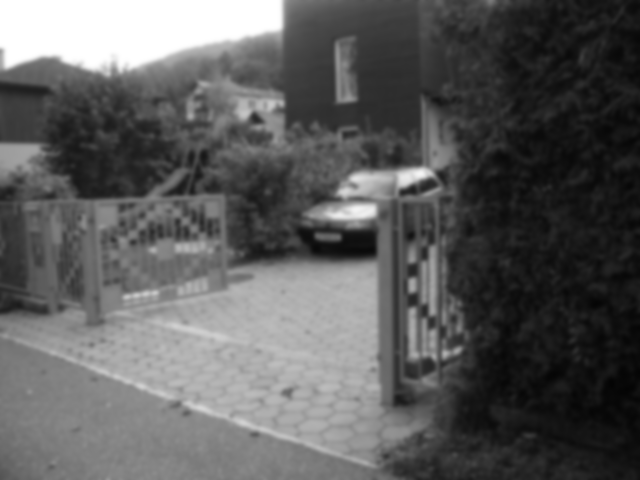
\includegraphics[width=\textwidth]{img/scaleSpaceTheory_2.png}
		\caption{$\sigma = 2$}
		\label{fig:scaleSpaceExample2}
	\end{subfigure}
	\begin{subfigure}[t]{0.3\textwidth}
		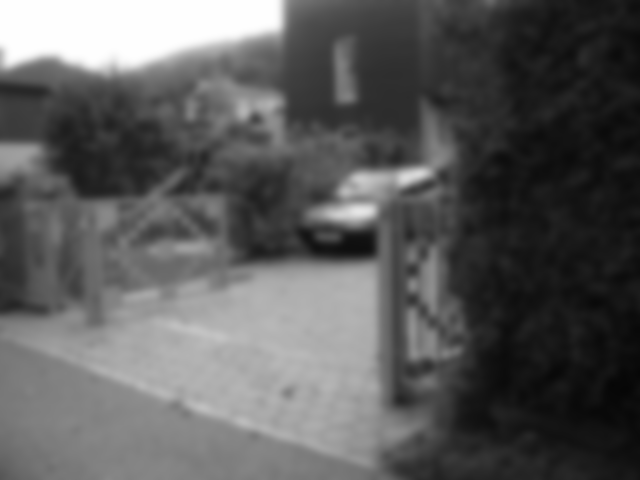
\includegraphics[width=\textwidth]{img/scaleSpaceTheory_4.png}
		\caption{$\sigma = 4$}
		\label{fig:scaleSpaceExample4}
	\end{subfigure}
	\begin{subfigure}[t]{0.3\textwidth}
		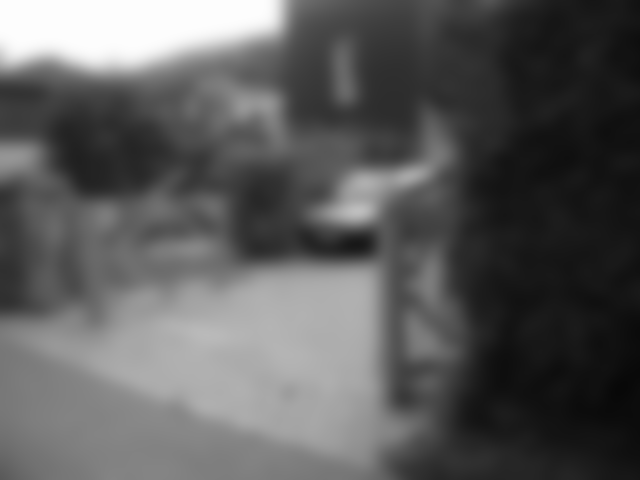
\includegraphics[width=\textwidth]{img/scaleSpaceTheory_8.png}
		\caption{$\sigma = 8$}
		\label{fig:scaleSpaceExample8}
	\end{subfigure}
	\begin{subfigure}[t]{0.3\textwidth}
		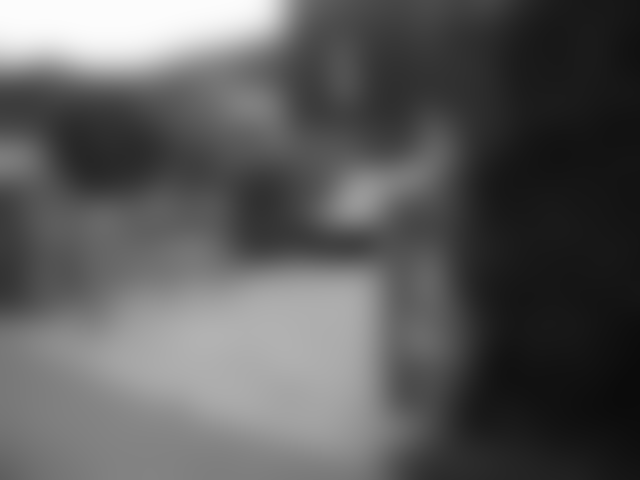
\includegraphics[width=\textwidth]{img/scaleSpaceTheory_16.png}
		\caption{$\sigma = 16$}
		\label{fig:scaleSpaceExample16}
	\end{subfigure}
	\caption{Example of a finite scale-space representation with scales $\sigma = 1,2,4,8,16$ of an image from the INRIA dataset (\Cref{sec:odDataset}).}
	\label{fig:scaleSpaceExample}
	\vspace{0.5cm}
	
	\begin{subfigure}[t]{0.23\textwidth}
		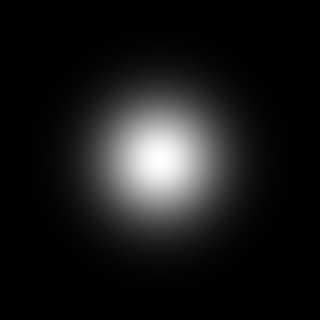
\includegraphics[width=\textwidth]{img/gaussianDerivative_0_0.png}
		\caption*{$G$}
	\end{subfigure}
	\vspace{2mm}	
	
	\begin{subfigure}[t]{0.23\textwidth}
		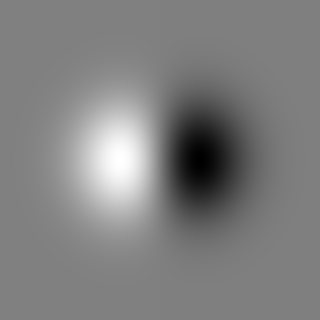
\includegraphics[width=\textwidth]{img/gaussianDerivative_1_0.png}
		\caption*{$G_{x}$}
	\end{subfigure}
	\begin{subfigure}[t]{0.23\textwidth}
		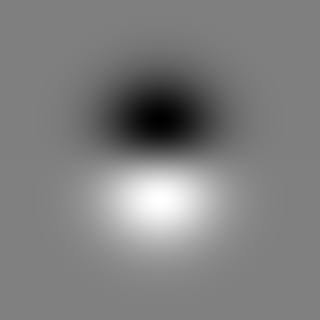
\includegraphics[width=\textwidth]{img/gaussianDerivative_0_1.png}
		\caption*{$G_{y}$}
	\end{subfigure}
	\vspace{2mm}
	
	\begin{subfigure}[t]{0.23\textwidth}
		
\includegraphics[width=\textwidth]{img/gaussianDerivative_2_0.png}
		\caption*{$G_{xx}$}
	\end{subfigure}
	\begin{subfigure}[t]{0.23\textwidth}
		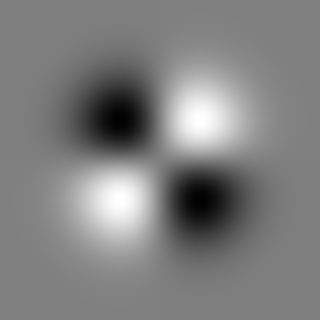
\includegraphics[width=\textwidth]{img/gaussianDerivative_1_1.png}
		\caption*{$G_{x y}$}
	\end{subfigure}
	\begin{subfigure}[t]{0.23\textwidth}
		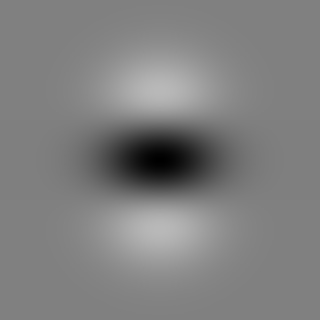
\includegraphics[width=\textwidth]{img/gaussianDerivative_0_2.png}
		\caption*{$G_{yy}$}
	\end{subfigure}
	\caption{Gaussian derivatives up to second order.}
	\label{fig:gaussianDerivatives}
\end{figure}

\section{Differential structure}
\label{sec:diffStructure}
When analysing an image, we are usually interested in the structure of the image. A typical approach to describing the structure is to compute the derivatives of the image up to the n'th order. Real world images are however usually filled with small-grained noise, which is why we often prefer to combine the derivative calculations with a smoothing of the image using a Gaussian filter. The details of this step are explained further in \Cref{sec:gaussianDerivatives}. The first order information, called the gradient, is described in \Cref{sec:gradientTheory}, and the second order information in the form of the shape index is described in \Cref{sec:shapeIndexTheory}.

\subsection{Gaussian derivatives}
\label{sec:gaussianDerivatives}

The \emph{Gaussian derivatives} $G_{x^m y^n}$, where $m$ is the order of derivations in the $x$-axis and $n$ is the order of derivations in the $y$-axis, are used for obtaining structural information from an image. \Cref{fig:gaussianDerivatives} illustrates the Gaussian derivatives up to second order.

The Gaussian derivatives are used for computing Gaussian derivative scale-space images $L_{x^m y^n}$:
\begin{align}
	L_{x^m y^n}(x,y;\sigma) &= G_{x^m y^n}(x,y;\sigma) \ast I(x,y)
\end{align}
We often compute the Gaussian derivatives analytically, and then convolve the image $I$ by the derived Gaussian filter. Given a Gaussian filter smaller than the image $I$, this ordering minimizes the number of calculations needed since we only compute one convolution with $I$.

In theory the Gaussian function has infinite support, but in practice one often uses the 3-sigma rule to determine the support radius of the Gaussian filter and hence the computational load of the convolution.

Since the Gaussian derivative scale-spaces are computed on a set of increasing scales, we need to compute all the needed derivatives for each scale. This give us a large amount of convolutions of the same image using various sizes Gaussian filters, which is computationally inefficient. Given these circumstances, we now describe an alternative and computationally cheaper way of computing the Gaussian derivative scale-spaces. The idea is to compute one smoothing per scale and then calculate all the derivatives at that scale using finite differences. We first define the central differences filter $f$:
%
\begin{align*}
	I_x &= \frac{\partial I}{\partial x} \approx f_x \ast I = \begin{bmatrix} -1 & 0 & 1\end{bmatrix} \ast I \\
	I_y &= \frac{\partial I}{\partial y} \approx f_y \ast I = \begin{bmatrix} -1 & 0 & 1\end{bmatrix}^\text{T} \ast I
\end{align*}
%
The combined $f_{x^m y^n}$-filter is simply made by convolving $m$ $f_x$-filters and $n$ $f_y$-filters in a chain. Substituting the Gaussian derivatives by the central differences convolved with a Gaussian filter give us:
%
\begin{align*}
	L_{x^m y^n}(x,y;\sigma) &= G_{x^m y^n}(x,y;\sigma) \ast I(x,y) \\
		&\approx f_{x^m y^n} \ast G(x,y;\sigma) \ast I(x,y) \\
		&= f_{x^m y^n} \ast L(x,y;\sigma)
\end{align*}
%
Since we have a nice set of increasing scales for our scale-space images, we are able to compute $L(x,y,\sigma_2)$ by using the previous scale space $L(x,y,\sigma_1)$ where $\sigma_2 > \sigma_1$ as described in \cite{tola2008fast}. The idea is to split up the smoothing into two operations and then use the associativity of convolution to use the previous scale-space image for the new smoothing:
%
\begin{align*}
	L(x,y;\sigma_2) &= G(x,y;\sigma_2) \ast I(x,y) \\
					&= (G(x,y;\sigma_\Delta) \ast G(x,y;\sigma_1)) \ast I(x,y),\hspace{1cm}\sigma_2 > \sigma_1 \\
					&= G(x,y;\sigma_\Delta) \ast L(x,y;\sigma_1) \\
			 \sigma_\Delta &= \sqrt{\sigma_2^2 - \sigma_1^2}
\end{align*}
%
Which give us the final equations for the alternative way of computing the Gaussian derivative scale-spaces.

\subsection{Gradient orientation and magnitude}
\label{sec:gradientTheory}
%
The \emph{gradient orientation} $\Theta \in [-\pi,\pi]$ is the orientation of the local first order derivatives. $\Theta$ is independent of the size of the derivatives, which is given by the \emph{gradient magnitudes} $M$. $\Theta$ and $M$ are defined in terms of the image derivatives as
%
\begin{align*}
\Theta &= \text{atan2}(L_y,L_x) \\
M &= \sqrt{L_x^2 + L_y^2}
\end{align*}
where atan2 is the arctangent function spanning the whole range of angles $[-\pi,\pi]$.
%
\Cref{fig:gradientOrientationTheory} illustrates the relationship between the gradient orientation, gradient magnitude, and $x$- and $y$-derivatives.
%
\begin{figure}[p]
	\centering
	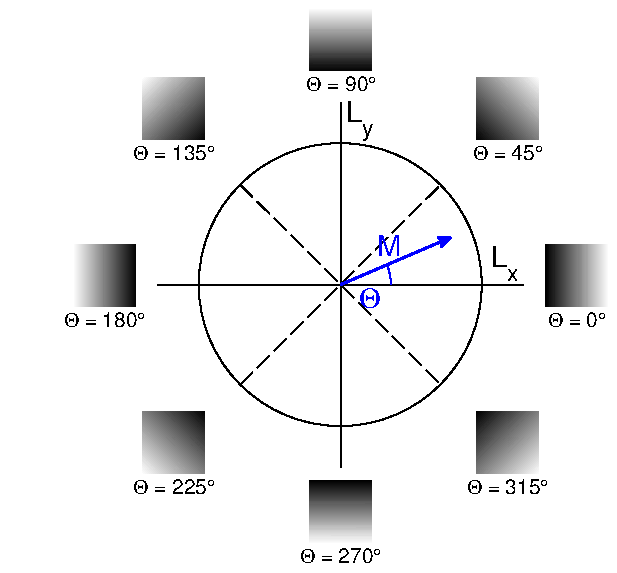
\includegraphics[width=0.63\textwidth,clip=true,trim=31 0 0 0]{img/gradientOrientationTheory.pdf}
	\caption{Gradient orientation and magnitude shown in the coordinate system $(L_x,L_y)$ of first order image derivatives.}
	\label{fig:gradientOrientationTheory}
	\vspace{0.5cm}	
	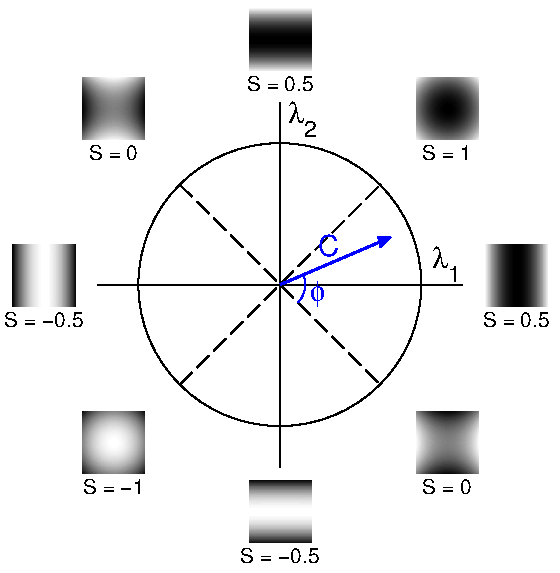
\includegraphics[width=0.63\textwidth,clip=true,trim=31 0 0 0]{img/shapeIndexTheory.pdf}
	\caption{Shape index and curvedness shown in the coordinate system $(\kappa_1,\kappa_2)$ of principal curvatures. The blue vector illustrates a shape index $S = \frac{2}{\pi} \phi$ and curvedness $C$, where $\phi$ is the signed angle between the vector and the line $\kappa_2 = -\kappa_1$. Note that the order of $\kappa_1$ and $\kappa_2$ does not matter, as shape index is independent of the orientation of the local geometry.}
	\label{fig:shapeIndexTheory}
\end{figure}

\subsection{Shape index and curvedness}
\label{sec:shapeIndexTheory}
%
The \emph{shape index} $S \in [-1,1]$ \cite{koenderink1992surface} is a scalar characterization of local second order derivatives. Like $\Theta$ and $M$, $S$ is independent of the size of the derivatives, which is given by the \emph{curvedness} $C$. Additionally the shape index is independent of orientation.

$S$ is defined by the orientation of the eigenvalues $\kappa_1$ and $\kappa_2$, also called the principal curvatures, of the local Hessian matrix $\nabla^2 L$. It can also be expressed by the local image derivatives:
%
\begin{align}
S &= \frac{2}{\pi} \Atan{\frac{\kappa_1 + \kappa_2}{\kappa_1 - \kappa_2}} \\
&= \frac{2}{\pi} \Atan{\frac{-L_{xx} - L_{yy}}{\sqrt{4 L_{xy}^2 + (L_{xx} - L_{yy})^2}}}
\end{align}
%
$C$ is defined by the size of $\kappa_1$ and $\kappa_2$, and can also be expressed by the image derivatives:
%
\begin{align}
C &= \sqrt{\frac{\kappa_1^2 + \kappa_2^2}{2}} \\
&= \frac{1}{\sqrt2} \sqrt{L_{xx}^2 + 2 L_{xy}^2 + L_{yy}^2}
\end{align}
%
\Cref{fig:shapeIndexTheory} illustrates the relationship between the principal curvatures, shape index and curvedness, as well as the geometry of various shape indices. As seen in the figure, $S$ ranges over light blobs ($S = -1$), ridges ($S = -0.5$), saddle points ($S = 0$), valleys ($S = 0.5$), and dark blobs ($S = 1$) with continuous deformations in between.
%
\section{Invariants and robustness}
When describing interest points and their local regions in real world images, we experience a lot of transformations of the actual physical objects. We are however interested in being able to describe the interest point without any (or a predefined set) of these transformations applied, in which case we have a better chance of recognizing the interest point in other images.

Apart from invariance to various transformations we also want to be robust to small changes in some of the transformations. This robustness should give us nearly equal descriptors despite having small errors in our estimation of the transformations.
In this section we will go through a list of transformations that we wish for our descriptor to be invariant and possibly also robust to.

\begin{table}[H]
	\centering
	\begin{tabular}{@{}l|ll@{}}
	%\toprule
	Measure & Rotation & Illumination \\
	\hline
	$\Theta$ & $\Theta - \theta $ & $\Theta$ \\
	$M$ & $M$ & $a M$ \\
	$S$ & $S$ & $S$ \\
	$C$ & $C$ & $a C$ \\
	%\bottomrule
	\end{tabular}
	\caption{The transformation of various measures by rotation and illumination. The derivations are included in \cref{apx:image_transformations}.}
	\label{tbl:measureInvariances}
\end{table}

\subsection{Translation}
The first transformation that we describe is translation. Translation occurs when images are taken from different positions and hence the interest points are translated in the image plane. Translation invariance is often achieved by combining a descriptor with an interest point detector which tells the descriptor where the interest points are located spatially in the image. Another approach is to use a sliding window technique in which a detection window is moved around the image trying to find a suitable matching position as in \cite{felzenszwalb2008discriminatively}. Translation invariance is almost always desired since even tiny vibrations at the time of capture can cause an object to change position in an image.

An interest point detector or a sliding window is only able to give an estimate of positions of interest points based on the detail available in the pixels of the image. We therefore also wish to have a descriptor which is robust to small changes in interest point positions allowing for a small error in detection point without having a large impact on the descriptor.

\subsection{Rotation}
Rotation naturally occurs when either the camera or the object in question is rotated. Even though a precise position is located, the outcome of descriptors with spatial pooling will be affected by rotation, if no efford is done to achieve rotational invariance. For SIFT-like descriptors the general approach to achieving rotational invariance is to estimate the direction of the feature and rotate the descriptor grid before computing the descriptor. Rotation invariance is often desired but not always needed, as in \cite{dalal2005histograms,felzenszwalb2008discriminatively} where only detection of pedestrians in upright positions is needed.

Looking at the differential measures $\Theta, M,~S,$ and $C$, we are able to derive the resulting measure under rotation by $\theta$. We have left out the details of the derivations here, but they can be found in \Cref{apx:rotation}. The final derived results are shown in \Cref{tbl:measureInvariances}. We see that both $M,~S,$ and $C$ are rotational invariant whereas $\Theta$ is rotated by the transformation angle $\theta$.
%
\subsection{Reflection}


\subsection{Illumination}
\label{sec:illumination}
Reference \Cref{apx:illumination} for $\Theta,~M,~S$, and $C$.
By using a small sigma for calculating the derivatives in the jet, we only use a small spatial area for the calculations which minimizes the risk of crossing a shadow edge. By combining multiple jets or shape indices into histograms we are able to calculate a descriptor across a shadow edge but still maintaining illumination invariance.

\subsection{Scale}
\label{sec:scaleInvariance}
Noget med scalespace \cite{griffin1997scale}.

\subsection{Perspective}
noget med ?



\section{Histograms}
\label{sec:histograms}

Histograms play an essential role in SIFT-like descriptors. They are used for aggregating gradient orientation (GO) and magnitude information over local areas. Traditionally histograms have been constructed using hard boundaries between bins; and descriptors have been constructed with hard boundaries between the local histogram areas of a descriptor.

These types of histograms are however neither robust to small interest point translation/detection errors or gradient orientations close to the bin boundaries. SIFT used a trilinear interpolation of the gradient magnitude based on the radial distance between the gradient orientation and the bin centers to cope with gradients close to the bin boundaries. In order to improve upon the robustness of the histograms, we here describe a histogram framework which is able to produce both ordinary (hard bounded) as well as smooth histograms based on locally orderless images (LOI), \cite{koenderink1999structure}.

The idea behind smooth histograms is to remove the sharp boundaries of ordinary histograms (bin boundaries). Given a position we wish to create a histogram for the surrounding local area/region of interest (ROI). This is done by letting all the values from the ROI contibute to all the bins of the histogram. The contribution of each value to each bin is dependent of the spatial distance to the chosen position, the distance between the value and the bin center (angular distance for GO histograms), and the value weight (typically gradient magnitude for GO histograms). Both distance weights are simple functions of a distance and hence we are able to compute ordinary sharp-bounded histograms by using box functions and smooth histograms by using Gaussian functions.

\citet{koenderink1999structure} define the LOIs from three scales: inner scale $\sigma$, tonal scale $\beta$, and outer scale $\alpha$. When applying the framework to our work, the inner scale corresponds to the feature scale (scale in scale-space), the tonal scale corresponds to the width of the histogram bin weight function, and the outer scale corresponds to the size of the ROI. The specifics of the histograms used in our work are explained in \Cref{eq:proposed_histogram}.
\mycomment[MSN]{How much theory here?}

Notes:
Given a domain in the interval $l \leq r$, we compute the histogram...
$H(\mu;\sigma,\beta,\alpha)$

\subsection{Periodic histograms}
When creating histograms of periodic domains, we need to take the periodicity into consideration. We specify the period between $l$ and $r$, where $l \leq r$.
The periodicity of the domain means that there are multiple distances between any two points. Since we are computing distance weight functions, we need to find the minimum distance $d_{wrap}$ from each point to each bin center in order to correctly compute the weight functions. This is done by a simple wrap-around using the known period of the domain as maximum distance:
\begin{align*}
	d_{wrap} = \min(d,(r - l)-d)
\end{align*}
where $d$ is the distance $x - \mu$ from a point $x$ to a bin center $\mu$, and $\min$ is the function that chooses the lowest of its arguments.

 \Cref{fig:1dFilterGaussianPeriodic,fig:1dFilterTrianglePeriodic,fig:1dFilterBoxPeriodic} show 1D examples of four periodic Gaussian, triangle and box filters respectively on the interval $[-1,1]$. Notice how the wrap-around affects the filters at both ends of the periods as expected.

\subsection{Renormalization}
When making histograms over a non-periodic domain, the weight function will be cropped by the histogram bounds $l$ and $r$. We therefore risk biasing the weights towards the central bins of the domain, since the cropped filters will have. In order to avoid this, we view the bins as probability densities, and hence the area under each bin's weight function has to integrate to 1. This is done by renormalizing the functions based on their areas. Given a filter function $f$ and a bin center $\mu$, for which $l \leq \mu \leq r$ we first calculate the integral bounds $a$ and $b$ followed by the actual area integral $A(\mu,\sigma)$ itself:
\begin{align*}
	a &= l - \mu,\hspace{1cm}
	b = r - \mu \\
	A(\mu,\sigma) &= \int_a^b f(x;\mu,\sigma)\,\text{d}x
\end{align*}
We notice that $a \leq 0 \leq b$. This area is simply used as the normalization constant of the bin centered in $\mu$ resulting in the probability density histogram $H_{pd}$:
\begin{align*}
	H_{pd}(\mu) = \frac{H(\mu)}{A(\mu,\sigma)}
\end{align*}
The calculations of $A(\mu,\sigma)$ for the Gaussian, triangle, and box filters are shown below in \Cref{sec:histogramsGaussianFilter,sec:histogramsTriangleFilter,sec:histogramsBoxFilter}.

\Cref{fig:1dFilterGaussianRenorm,fig:1dFilterTriangleRenorm,fig:1dFilterBoxRenorm} show 1D examples of four renormalized Gaussian, triangle, and box filters respectively on the interval $[-1,1]$. Notice how the two weight functions of the outer-most bins have higher peaks than the central bins in order to integrate to 1 when being cut off at the interval bounds. For periodic histograms the renormalization step is excluded since no cut off of the filters occurs.
\todo{Decide what to do with the poor box illustration}


\begin{figure}
	\centering
	\begin{subfigure}[t]{0.32\textwidth}
		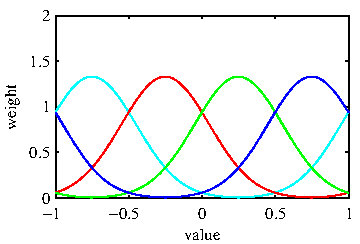
\includegraphics[width=\textwidth]{img/binFilterGaussianPeriodic.pdf}
		\caption{Periodic Gaussian}
		\label{fig:1dFilterGaussianPeriodic}
	\end{subfigure}
	\begin{subfigure}[t]{0.32\textwidth}
		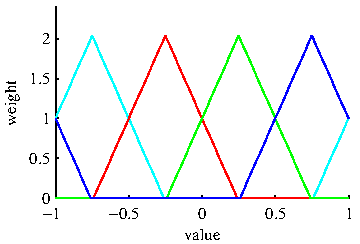
\includegraphics[width=\textwidth]{img/binFilterTrianglePeriodic.pdf}
		\caption{Periodic Triangle}
		\label{fig:1dFilterTrianglePeriodic}
	\end{subfigure}
	\begin{subfigure}[t]{0.32\textwidth}
		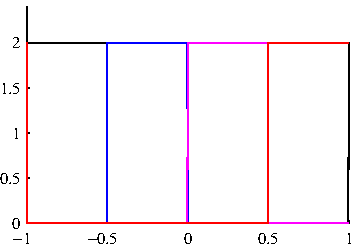
\includegraphics[width=\textwidth]{img/binFilterBoxPeriodic.pdf}
		\caption{Periodic box}
		\label{fig:1dFilterBoxPeriodic}
	\end{subfigure}
	\begin{subfigure}[t]{0.32\textwidth}
		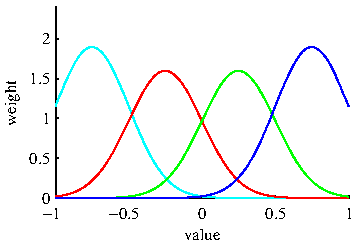
\includegraphics[width=\textwidth]{img/binFilterGaussianRenorm.pdf}
		\caption{Renorm. Gaussian}
		\label{fig:1dFilterGaussianRenorm}
	\end{subfigure}
	\begin{subfigure}[t]{0.32\textwidth}
		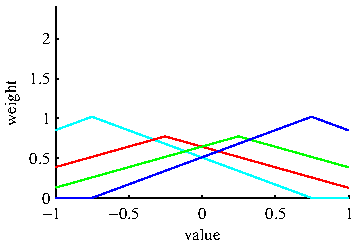
\includegraphics[width=\textwidth]{img/binFilterTriangleRenorm.pdf}
		\caption{Renorm. triangle}
		\label{fig:1dFilterTriangleRenorm}
	\end{subfigure}
	\begin{subfigure}[t]{0.32\textwidth}
		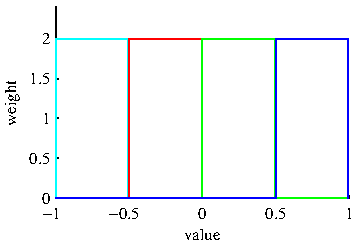
\includegraphics[width=\textwidth]{img/binFilterBoxRenorm.pdf}
		\caption{Renorm. box}
		\label{fig:1dFilterBoxRenorm}
	\end{subfigure}
	\caption{Examples of periodic and renormalized 1D Gaussian, triangle, and box functions. Each figures contains four filters centered at values $-0.75$, $-0.25$, $0.25$, and $0.75$ and with $\sigma = \nicefrac{1}{2}$.}
	\label{fig:1dFilters}
\end{figure}

\begin{align}
\end{align}

\subsection{Gaussian filter}
\label{sec:histogramsGaussianFilter}
\todo{Should the following 3 subsections be moved to appendx?}

The 1-dimensional Gaussian filter with variance $\sigma$ is defined as:
%
\begin{align*}
G(x;\sigma) = \frac{1}{\sqrt{2\pi} \sigma}
\exp\left( -\frac{x^2}{2 \sigma^2} \right)
\end{align*}
%
The definite integral of $G(x;\sigma)$ from $a$ to $b$ cannot be expressed by an elementary function. Instead we can use the non-elementary error function, defined as $\mathrm{erf}(b) = \frac{2}{\sqrt{\pi}} \int_0^b \exp(-x^2) \,\mathrm dx$, which can be computed by its Taylor series. First we show an intermediate result using the substitution $u = \sqrt{k} x$ with $\mathrm du = \sqrt{k} \mathrm dx$:
%
\begin{align*}
\int_0^b \exp(-k x^2) \,\mathrm dx
&= \frac{1}{\sqrt{k}} \int_0^{\sqrt{k}b} \exp(-u^2) \,\mathrm du \\
&= \frac{1}{\sqrt{k}} \frac{\sqrt{\pi}}{2} \mathrm{erf} \left( \sqrt{k} b \right)
\end{align*}
%
We use this to compute $\int_a^b G(x;\sigma) \,\mathrm dx$:
%
\begin{align*}
\int_a^b G(x;\sigma) \,\mathrm dx
&= \frac{1}{\sqrt{2\pi} \sigma} \int_a^b \exp\left( -\frac{x^2}{2 \sigma^2} \right) \,\mathrm dx \\
&= \frac{1}{\sqrt{2\pi} \sigma} \left( \int_0^b \exp\left( -\frac{x^2}{2 \sigma^2} \right) \,\mathrm dx - \int_0^a \exp\left( -\frac{x^2}{2 \sigma^2} \right) \,\mathrm dx \right) \\
&= \frac{1}{\sqrt{2\pi} \sigma} \frac{\sqrt{\pi}}{2} \sqrt{2} \sigma \left(
\mathrm{erf} \left( \frac{1}{\sqrt{2} \sigma} b \right) -
\mathrm{erf} \left( \frac{1}{\sqrt{2} \sigma} a \right) \right) \\
&= \frac{1}{2} \left(
\mathrm{erf} \left( \frac{b}{\sqrt{2} \sigma} \right) -
\mathrm{erf} \left( \frac{a}{\sqrt{2} \sigma} \right)
\right)
\end{align*}
%
The $n$-dimensional Gaussian filter with variances $\boldsymbol{\sigma} = [\sigma_1, ..., \sigma_n]^T$ is defined as the product of $n$ 1-dimensional filters:
%
\begin{align*}
G(\mathbf{x};\boldsymbol{\sigma})
&= \prod_i G(x_i;\sigma_i) \\
&= \frac{1}{(2\pi)^\frac{n}{2} \prod_i \mathbf{\sigma}_i}
\exp\left( -\sum_i \frac{x_i^2}{2 \sigma_i^2} \right)
\end{align*}
%
With this definition we disallow arbitrary covariances as it does not make sense for a binning function. Note that the factors of $G(\mathbf{x};\boldsymbol{\sigma})$ contain distinct variables. Thus its definite integral from $a_i$ to $b_i$ in each dimension is simply the product of the definite integrals for each dimension:
%
\begin{align*}
\int_{a_i}^{b_i} \dots \int_{a_n}^{b_n} G(\mathbf{x},\boldsymbol{\sigma}) \,\mathrm d{x_n} \dots d{x_i}
&= \prod_i \int_{a_i}^{b_i} G(\mathbf{x},\boldsymbol{\sigma}) \,\mathrm d{x_i} \\
&= \prod_i \frac{1}{2} \left(
\mathrm{erf} \left( \frac{b_i}{\sqrt{2} \sigma_i} \right) -
\mathrm{erf} \left( \frac{a_i}{\sqrt{2} \sigma_i} \right)
\right)
\end{align*}
%
\subsection{Triangle filter}

\subsection{Box filter}


\section{Binary classification measures}

We base our performance measure on the confusion matrix shown in \Cref{tbl:confusion_matrix}. Using a ground truth (or golden standard), which tells us if two points in the two images in question indeed correspond to one another, we are able to classify each match result into one of the four cells of the confusion matrix. From the four outcomes we define the following three measurements: \emph{recall} ($\TPR$), \emph{fall-out} ($\FPR$), and \emph{1-precision} ($\OMP$) as shown in \Cref{eq:fpr,eq:tpr,eq:omp} respectively.
\begin{align}
	\label{eq:fpr}
	\FPR &= \frac{\FP}{\FP + \TN} \\
	\label{eq:tpr}
	\TPR &= \frac{\TP}{\TP + \FN} \\
	\label{eq:omp}
	\OMP &= \frac{\FP}{\FP + \TP}
\end{align}
Where $\TP,\FP,\TN,~\text{and}~\FN$ are the number of matches placed in each of the four cells of the confusion matrix.

As mentioned above, the threshold $t$ is required in order to classify the matches. In order to get a performance measure independent of the choice of $t$, we vary $t$ across all unique ratios and obtain the measurements $\FPR,\TPR,$ and $\OMP$.

From these three measurements we draw the \ROC-curve and the \PR-curve defined as recall vs. fall-out and recall vs. 1-precision respectively. Integrating these curves gives us the area under the curve (AUC) for \ROC\ or \PR, where a high AUC means that our descriptor is good at separating the matches that correspond to one another from those that don't.

\begin{table}[tb]
	\centering
	\bgroup
	\def\arraystretch{1.5}
	\begin{tabular}{|l|c|c|}
		\cline{2-3}
		\multicolumn{1}{c|}{} & Condition positive & Condition negative \\ \hline
		Assigned positive & \cellcolor{green!25}True Positive (TP) & \cellcolor{red!25}False Negative (FN)  \\ \hline
		Assigned negative & \cellcolor{red!25}False Positive (FP) & \cellcolor{green!25}True Negative (TN) \\ \hline
	\end{tabular}
	\egroup
	\caption{Confusion matrix for postive/negative classification}
	\label{tbl:confusion_matrix}
\end{table}

\section{Detectors}
Detectors, combined with scale space, DoG chosen as our detector

\subsection{Difference of Gaussian}
DoG detector

\begin{figure}[tb]
	\centering
	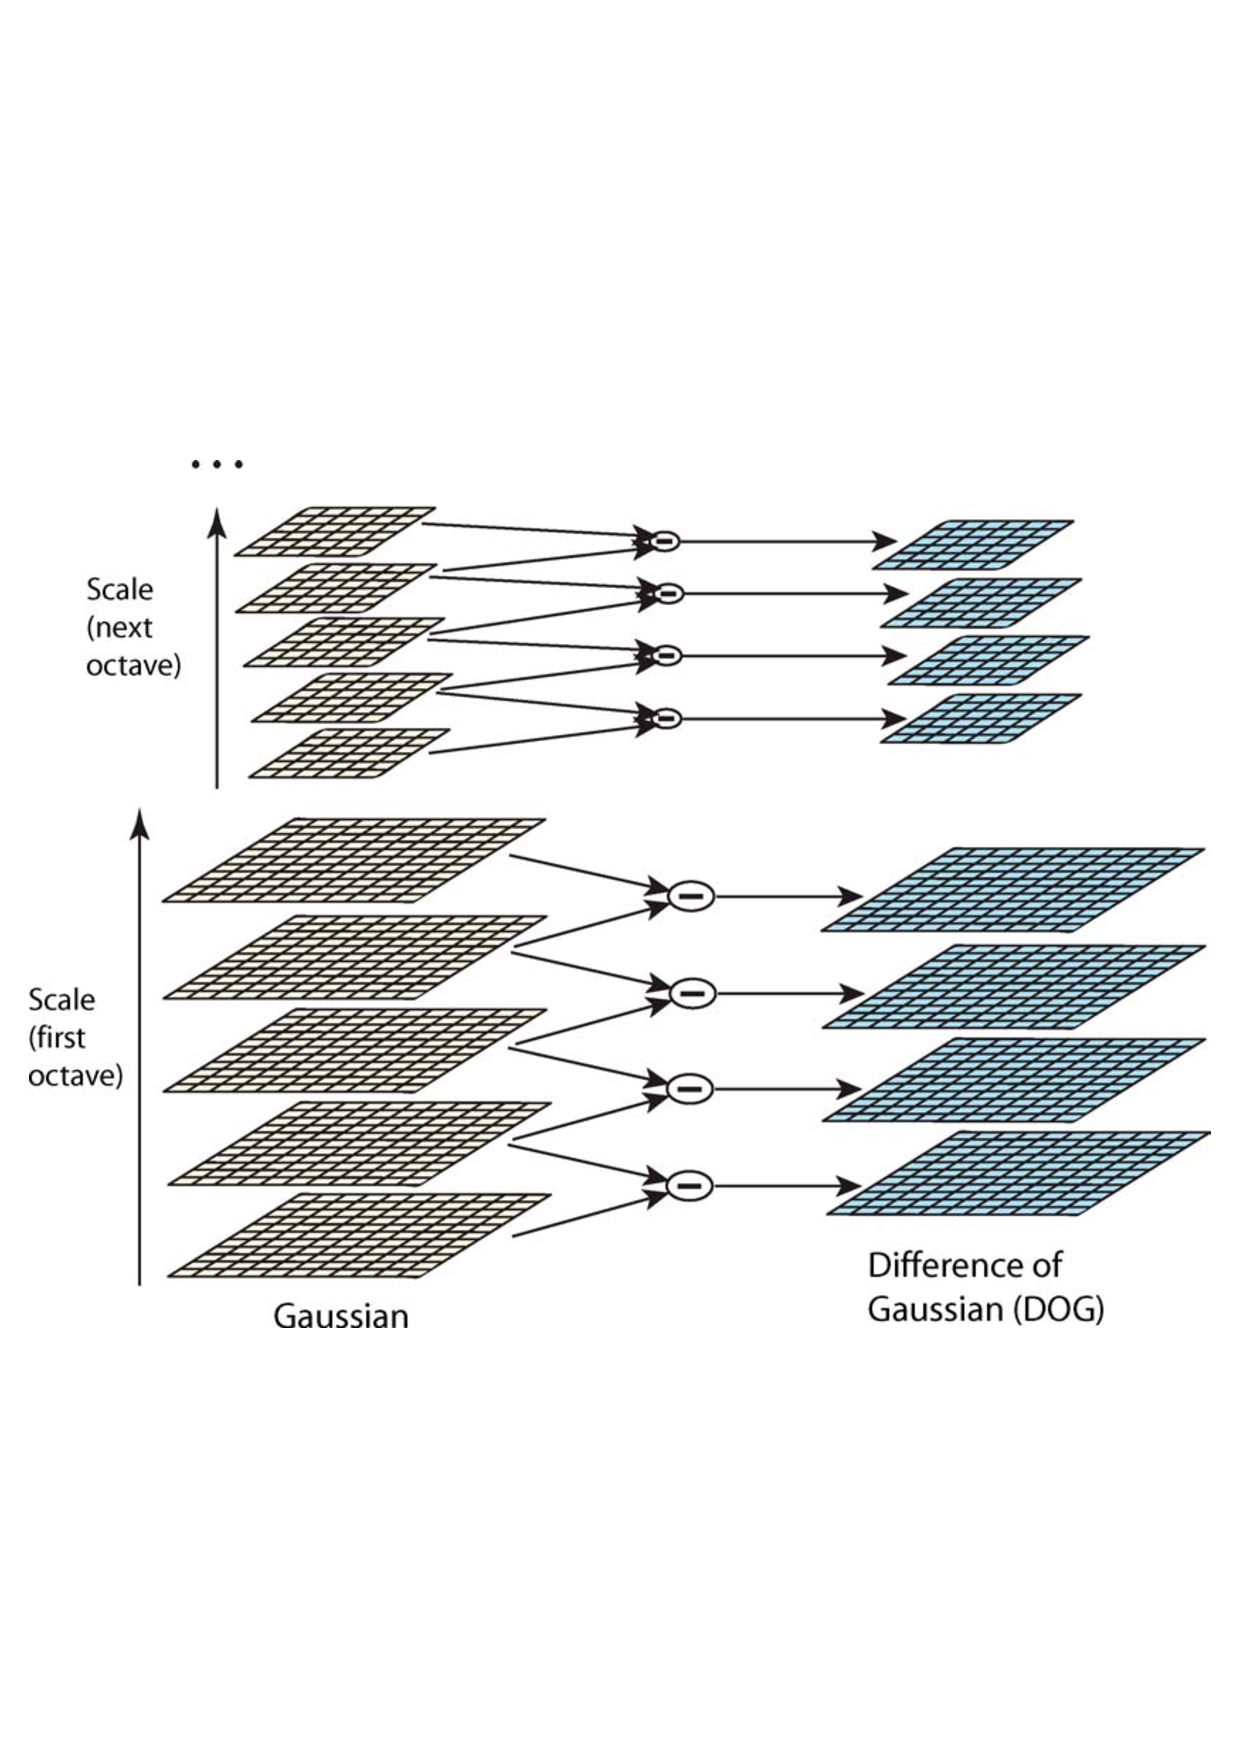
\includegraphics[width=\textwidth,clip=true,trim=0 200 0 220]{img/SIFT_dogspaces.pdf}
	\caption{Reproduced DoG scalespace figure \cite[figure 1,pp. 95]{lowe2004distinctive}. Original caption: For each octave of scale space, the initial image is repeatedly convolved with Gaussians to produce the set of scale space images
shown on the left. Adjacent Gaussian images are subtracted to produce the difference-of-Gaussian images on the right. After each octave, the
Gaussian image is down-sampled by a factor of 2, and the process repeated.}
	\label{fig:dogSpaces}
\end{figure}

\section{Descriptors}

Other descriptors as described in the literature study. We choose SIFT to compare against.

\subsection{SIFT}

Gradients of an image are often used to describe the region around interest points, since they describe the changes in intensities in the image plane.
The \emph{scale-invariant feature transform} (SIFT) descriptor
\cite{lowe2004distinctive} is the most popular descriptor based on this
approach. It works by dividing the image regions surrounding interest
points into square cells and constructing a histogram of gradient
orientations for the pixels in each cell. The interest points are detected
using a multi-scale DoG detector. By computing the gradient orientations
at detection scale, the descriptor becomes scale invariant. The descriptor
is also rotation invariant as the cell grid is rotated according to the
dominating gradient orientation. Finally the descriptor achieves illumination
invariance by normalizing the histograms. The SIFT descriptor uses a grid of
$4 \times 4$ cells each consisting of $4 \times 4$ pixels, with 8 histogram
bins for each cell. This results in a dimensionality of $4 \times 4 \times 8 =
128$.


\subsection{HOG}

The \emph{Histograms of Oriented Gradient} (HOG) descriptor is another
alternative to SIFT proposed in \cite{dalal2005histograms} for pedestrian
detection. Contrary to SIFT which is computed individually at specified
interest points, the HOG descriptors are computed in a dense grid over a
detection window and each block descriptor is a part of a larger descriptor
usually trained using an SVM. The Gradients are first computed using simple
1D masks. Secondly magnitude and spatially weighted histograms of the
orientations (0-180$^{\circ}$) of the gradients are computed for spatial
regions named cells\todo{Add note about interpolation of votes}. The cells are
then grouped together into blocks of cells for normalization to accomodate
for local illumination changes. These blocks can either be rectangular with
rectangular cells (R-HOG), or circular using a log-polar partitioning as the
DAISY descriptor. The normalization is performed using either the L2-norm,
a clipped and re-normalized L2-norm, or the square root of the L1-norm for
best performance. HOG descriptors are able to work directly on RGB images
unlike the original SIFT descriptor. This is done by computing the gradients
for each colour channel and choosing the gradient with the highest magnitude
for each pixel. For R-HOG the optimal bin number is found to be 9, optimal
block size $3\times3$ cell blocks and optimal cell size $6\times6$ pixels
with block spacing 8.\todo{Should optimal parameters for C-HOG be mentioned?}
Furthermore parts models using the HOG descriptor have been developed
\cite{felzenszwalb2008discriminatively} in order to improve upon the accuracy
of object detection.

%
%\section{Sliding window}
%
%\section{Spatial pooling schemes}
%
%\section{Normalization (local)}
%
%\section{Rotational invariance}
%
%\section{Histograms}
%
%\section{PCA}
%
%\section{Gradient orientation}
%
%\section{$k$-Jets}
%
%\section{Shape index}

\subbibliography

\end{document}
